\cleardoublepage

\chapter{Study 4}
\label{res:wle}

\cleardoublepage

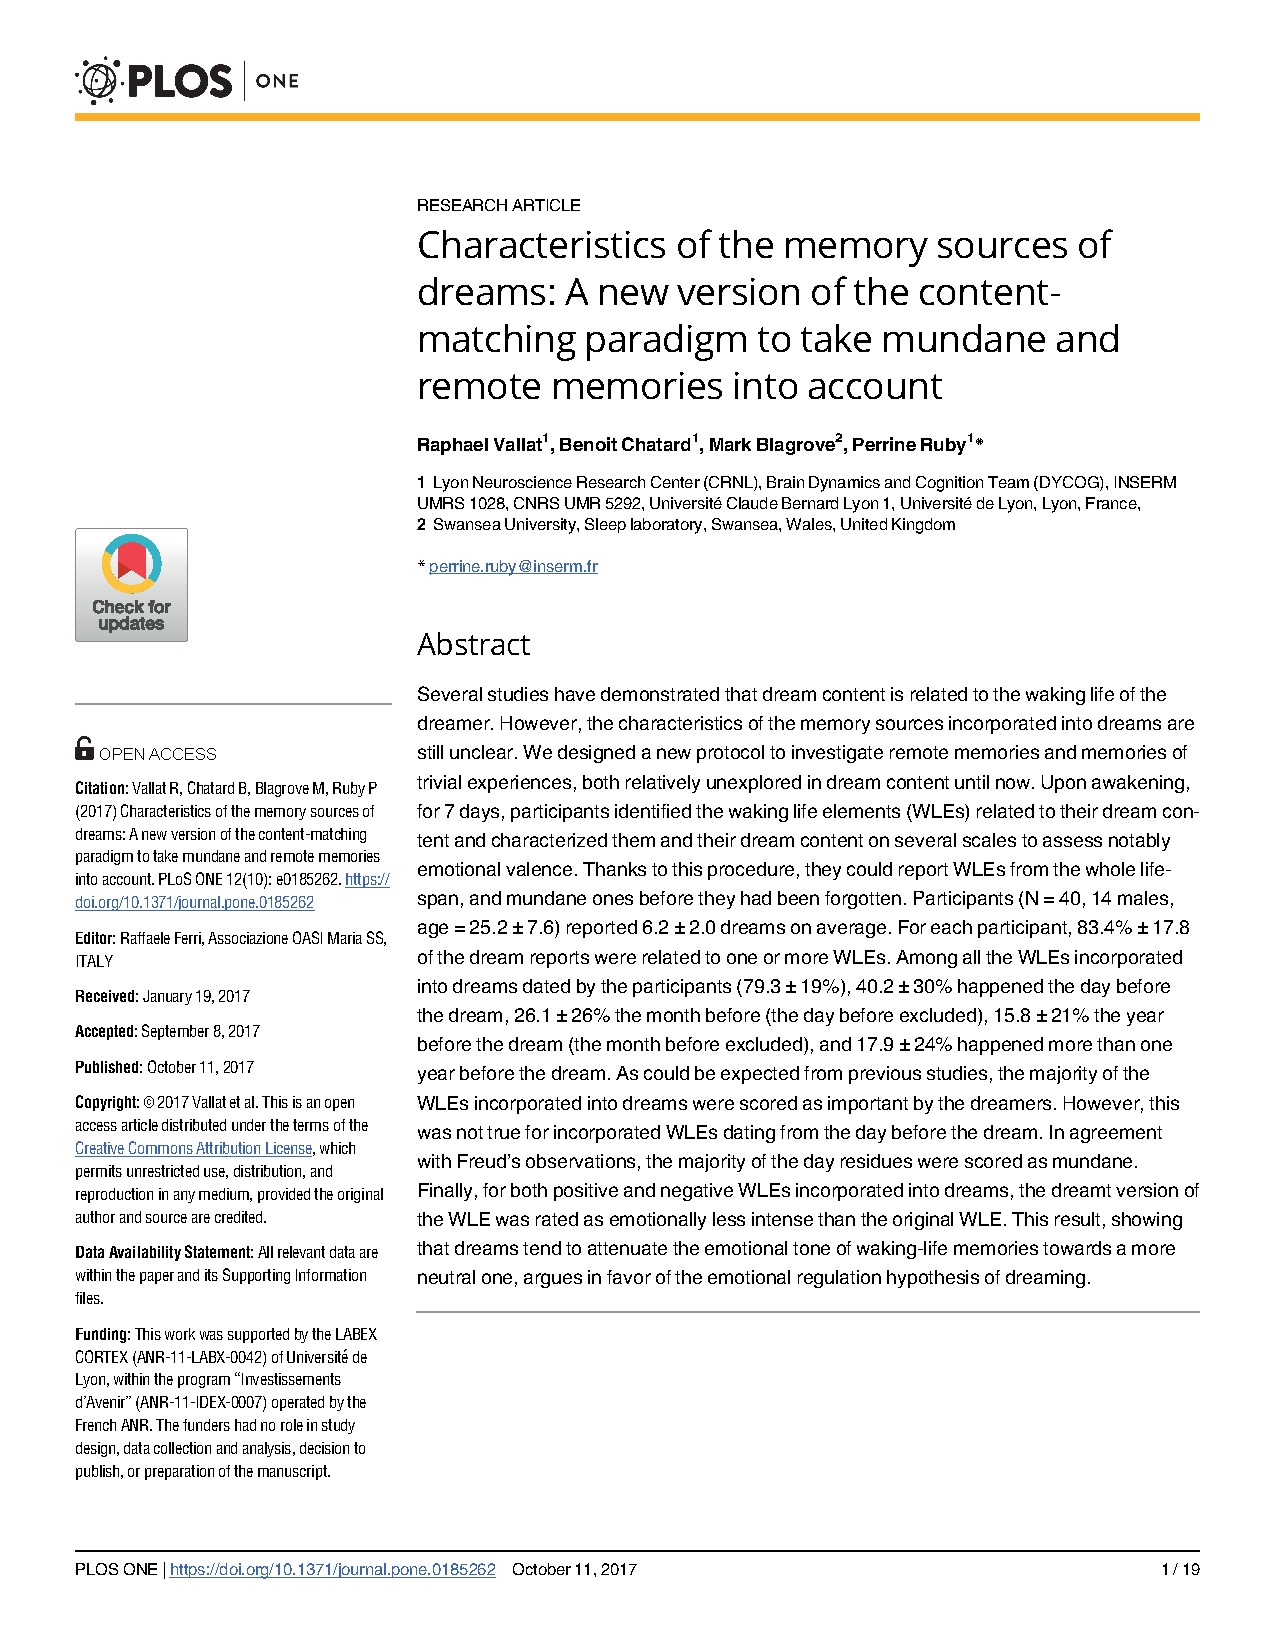
\includepdf[pages=-, pagecommand={\thispagestyle{plain}}]{Articles/Vallat_2017_PlosOne.pdf}

\cleardoublepage

\subsection*{Supplementary materials}
\label{res:wle:supp}
\vspace*{1cm}

\begin{figure}[htbp]
	\includegraphics[width=0.72\textwidth]{Fig/Results/WLE/S1_Fig.png}
	\caption*{\textbf{S1 Fig. Concerns reported in the initial questionnaire.} Concerns were distributed in 7 thematic categories. The number of concerns per categories are represented in pink. Red bars illustrate the percentage of concerns from one category that were incorporated into dreams during the 7-days experiment.}
\end{figure}

\vspace*{3cm}

\begin{figure}[htbp]
	\includegraphics[width=\textwidth]{Fig/Results/WLE/S2_Fig.png}
	\caption*{\textbf{S2 Fig. Distribution of the scores for all the WLEs incorporated into dreams and day-residues only} (see S2 Table for the figures).}
\end{figure}

\FloatBarrier

\clearpage

\textbf{S1 Table. Examples of waking life elements incorporated into dreams.} \\
\noindent\rule{\textwidth}{0.4pt}
\textbf{Old, important and emotionally negative WLE} \\
S1 | Valence = 2 ; Importance = 7 ; Dream valence = 5 \\
Dream report: \q{I am with an ex-girlfriend in my dream, we get along together very well} \\
WLE description: \q{We broke up several years ago in a difficult situation and none of us had given sign of life since.} \smallskip

S29 | Valence = 2 ; Importance = 10 ; Dream valence = 1 \\
Dream report: \q{I descend into another world to pick up my aunt and realize that it is not possible - I feel a deep anguish and I am cold} \\
WLE description: \q{My aunt passed away 3 months ago and I miss her terribly. I know she will not come back, but some days I still hope it will happen.} \smallskip

S35 | Valence = 2 ; Importance = 10 ; Dream valence = 3 \\
Dream report: \q{In my dream I saw my ex-girlfriend and her new partner. Suddenly, I felt really angry and started to push them down the stairs. They fell down and I shout at them.} \\
WLE Description: \q{Three years ago I bumped into them in the streets and was particularly unkind to them.} \smallskip

\textbf{Old, important and emotionally positive WLE} \\
S6 | Valence = 10 ; Importance = 10 ; Dream Valence = 10 \\
Dream report: \q{I was comforting two twins sisters that just got fired from the religious association I was working in several years ago.} \\
WLE description: \q{It reminded me of the responsibility I used to have there.} \smallskip

S19 | Valence = 10 ; Importance = 10 ; Dream Valence = 10 \\
Dream report: \q{I am working at my shop with my employee and my friend F* with whom I get along very well} \\
WLE description: \q{F* is an old school friend. At the time we were always together and for me he was almost part of the family} \smallskip

\textbf{Mundane and feebly emotional day-residues} \\
S3 | Valence = 5 ; Importance = 1 ; Dream valence = 6 \\
Dream report: \q{I was in an unknown house with two friends and a talking Koala.} \\
WLE description: \q{It reminded me of the talking raccoon in the movie Guardian of the Galaxy that I watched the day before.} \smallskip

S15 | Valence = 5 ; Importance = 1 ; Dream valence = 5 \\
Dream report: \q{I am in the supermarket looking for a dishwasher.} \\
WLE description: \q{Yesterday I saw on the internet a picture of the proper way to load dishes in a dishwasher.} \smallskip

S25 | Valence = 5 ; Importance = 1 ; Dream valence = 5 \\
Dream report: \q{In my dream I was creating magical creatures in order to destroy something}. \\
WLE description: \q{The creatures reminded me of the ones in the video game I played for several hours the day before.} \smallskip

S38 | Valence = 5 ; Importance = 1 ; Dream valence = 5 \\
Dream report: \q{I was in a house with a small swimming-pool.} \\
WLE description: \q{The swimming-pool was very similar to the one I saw yesterday in a park. The shape, depth and color were the same.} \smallskip

\textbf{Important and emotionally intense day-residues} \\
S40 | Valence = 1 ; Importance = 10 ; Dream Valence = 1 \\
Dream report: \q{I was at work, struggling to fix several mistakes made by my boss. At the end of the day, I took the blame and got fired.} \\
WLE description: \q{Yesterday there was a problem in my company after a client requested a sudden change.} \smallskip

S33 | Valence = 2 ; Importance = 8 ; Dream Valence = 4 \\
Dream report: \q{My father offers me a sewing machine. I realize that I already have this model.} \\
WLE Description: \q{My father is a recurring concern and we talked yesterday about his health. Also, yesterday I thought that I should sew this week-end.} \smallskip

S29 | Valence = 10 ; Importance = 10 ; Dream Valence = 10 \\
Dream report: \q{I was talking to several persons at the university and each time I tried to say only positive things in order to make them happy.} \\
WLE description: \q{Yesterday I thought that I should really stop being always negative and doubtful. In my dream it felt as if I put into practice this.} \smallskip

S19 | Valence = 10 ; Importance = 10 ; Dream Valence = 10 \\
Dream report: \q{In my dream there was this cartoon character that I really like.} \\
WLE description: \q{Yesterday I watched a really good new cartoon movie.} \\
\noindent\rule{\textwidth}{0.4pt}

\begin{table}[htb]
    \caption*{\textbf{S2 Table. Distribution of the score given to WLEs incorporated into dreams, for all WLEs (bold) and day-residues only.} For emotional valence, Low = negative and High = positive. Emotional intensity is rated on a 1-to-4 scale (see Methods). Neutral = medium emotional intensity.}
    \resizebox{\textwidth}{!}{%
    \begin{tabularx}{\textwidth}{Xlll}
    \toprule
    Characteristics                   & Low (\%)                    & Neutral (\%)          & High (\%)             \\ \midrule
    Frequency (Rare – Daily)          & \textbf{53.5 ± 22.3}        & \textbf{12.4 ± 11.4}  & \textbf{34.2 ± 24.2}  \\
                                      & 52.1 ± 33                   & 16.2 ± 25             & 31.7 ± 35             \\
    Familiarity (New – Familiar)      & \textbf{33.6 ± 21.7}        & \textbf{9.9 ± 14.5}   & \textbf{56.5 ± 23}    \\
                                      & 43 ± 37                     & 14.2 ± 25             & 42.9 ± 37             \\
    Emotional valence (Neg. – Pos.)   & \textbf{28.1 ± 20.9}        & \textbf{26.6 ± 25.3}  & \textbf{45.3 ± 26.2}  \\
                                      & 23.9 ± 28                   & 35.9 ± 34             & 40.2 ± 37             \\
    Importance                        & \textbf{34.4 ± 23.6}        & \textbf{12 ± 12.7}    & \textbf{53.5 ± 22.9}  \\
                                      & 48.2 ± 37                   & 12.2 ± 25             & 39.6 ± 38             \\
    Current concern                   & \textbf{56.6 ± 25.1}        & \textbf{9 ± 13.8}     & \textbf{34.4 ± 21.6}  \\
                                      & 57.8 ± 37                   & 9.1 ± 21              & 33.1 ± 33             \\
    Emotional intensity               & \textbf{42.5 ± 25.4}        & \textbf{32.9 ± 24.4}  & \textbf{24.6 ± 23.4}  \\
                                      & 52.6 ± 38                   & 24.9 ± 32             & 22.5 ± 33             \\ \bottomrule
    \end{tabularx}%
    }
\end{table}

\begin{table}[htb]
    \caption*{\textbf{S3 Table. Characteristics of the WLEs incorporated into dreams that happened 6 to 9 days before the dreams (n=36)}. Except for emotional intensity, Neutral (\%) refers to the percentage of WLEs with a score of 5. For emotional valence, Low = negative and High = positive. Emotional intensity is rated on a 1-to-4 scale (see Methods). Neutral = medium emotional intensity.}
    \resizebox{\textwidth}{!}{%
    \begin{tabularx}{\textwidth}{Xllll}
    \toprule
    Characteristics                 & Mean Score      & Low (\%)  & Neutral (\%) & High (\%) \\ \midrule
    Frequency (Rare – Daily)        & 4.1 ± 2.9       & 49.3 ± 48 & 18.6 ± 37    & 32.1 ± 42 \\
    Familiarity (New – Familiar)    & 5.2 ± 3.0       & 38.1 ± 43 & 25.2 ± 42    & 36.7 ± 42 \\
    Emotional valence (Neg. – Pos.) & 5.4 ± 2.1       & 24.6 ± 36 & 22.5 ± 39    & 52.9 ± 46 \\
    Importance                      & 5.7 ± 3.0       & 21.9 ± 34 & 19.5 ± 31    & 58.6 ± 39 \\
    Current concern                 & 5.1 ± 3.4       & 39.3 ± 40 & 8.6 ± 27     & 52.1 ± 40 \\
    Emotional intensity             & 1.4 ± 1.3       & 56.1 ± 46 & 31.8 ± 41    & 12.1 ± 29 \\ \bottomrule
    \end{tabularx}%
    }
\end{table}

% Table column width
\newcolumntype{b}{>{\hsize=0.35\textwidth}X}

\begin{table}[htb]
    \caption*{\textbf{S4 Table. Distribution (\%) of mundane WLEs incorporated into dreams according to their temporal remoteness.} Each time category mutually excludes the previous ones (e.g. month before excludes day before the dream).}
    \resizebox{\textwidth}{!}{%
    \begin{tabularx}{\textwidth}{bXXXX}
    \toprule
                                                        & Day before & Month before & More than a month & Not dated \\ \midrule
    Importance < 5, n=196                               & 43.4       & 19.9         & 20.4              & 16.3      \\
    Importance = 1, n=96                                & 52.1       & 17.7         & 17.7              & 12.5      \\
    Importance = 1 and emotional intensity = Low, n=70  & 60         & 20           & 8                 & 12        \\ \bottomrule
    \end{tabularx}%
    }
\end{table}

\subsubsection*{Supplementary results: distribution of the scores }
For each characteristic, the percentage of WLEs with a rating inferior, equal and superior to 5 was computed. A visual inspection of S2 Table shows that if we compare the distribution of the scores for all the WLEs incorporated into dreams and day-residues only, the distributions differ for familiarity, importance, and emotional valence and intensity. As compared to all WLEs incorporated into dreams, for day-residues only we observed a greater percentage of WLEs scored as feebly familiar, emotionally neutral, feebly important and feebly emotionally intense (S2 Fig).

\subsubsection*{Supplementary discussion}
\paragraph{The concern-related dimension of WLEs incorporated into the dreams}

According to the dreamers’ scoring, the WLEs incorporated into dreams are not predominantly concern-related (Table 2). This result is coherent with the experimenters’ assessment of the incorporation of current concerns into dreams taking the initial questionnaire into account. We found that in average 23\% of the dream reports of each subjects incorporated a current concern. Reciprocally, on average for each subject only 25\% of the concerns listed in the initial questionnaire were incorporated into a dream report during the 7 days of the experiment. Previous studies reported a larger percentage of dreams in relation with the dreamers’ current concerns. For example, \citet{schwartz_sleep_2002}, who used an automatic analysis of words on 1770 dreams of the first author found that 35\% of the dreams were considered related to current concerns. The great heterogeneity between studies may come from different definitions of the term \emph{concerns} and from different methods (if close friends and family were considered as concerns, the \% of dreams related to concerns would be much higher in our study). Our results show that when listed a priori (i.e. before dreams content analysis), current concerns are not as represented in dreams as would be expected from the dominant hypothesis saying that \q{much of it tends to revolve around a relative handful of personal concerns} \citep{domhoff_studying_2008}.

\paragraph{The characters and places incorporated into the dreams}

At least one external character was reported for nearly all remembered dreams. The mean number of characters per dream was slightly above with the norm (2.6 in \citealp{hall_content_1966}). This results is most likely due to several methodology differences: in Hall \& Van de Castle system, rating was done a posteriori by an external judge, who would consider groups of characters not individually named (e.g. a couple, a group of 3 children) as one character. In our study, the number of characters was assessed by the dreamer and considering each characters of the dreams as one individual. Regarding familiar existing persons (Fig 2) our results even if a little higher, are also coherent with the norm (familiar characters, 45\% in males and 58\% in females in \citealp{hall_content_1966}). However, in our data close family and friends appeared to be more represented than in the normative study (family, 9\% in males, 14\% in females; relatives, 2\% in males, 4\% in females in \citealp{hall_content_1966})

Regarding places, in our study participants reported nearly twice as much places (2.3 ± 1.5) as in the norm (average n° of settings per dream, 1.3 in \citealp{hall_content_1966}) and nearly half of these places were unknown (Fig 2) which is far more than the norm (unfamiliar, 14\% \citealp{hall_content_1966}). Finally, we observed a little less familiar places (familiar, 33\% \citealp{hall_content_1966}) and a little less mixed places (questionable, 40\% \citealp{hall_content_1966}). It is important to keep in mind that in our study the dreamers rated their own dreams while in \citet{hall_content_1966} an external rating was used. The two methods may yield divergent results \citep{sikka_i_2014}.
